% answers.tex —— 2004 年·普通高等学校春季招生考试·安徽卷理科 · 参考答案与详细解析片段
% 由 tools/generate_projects.py 依来源总账自 2004/2004_数学真题_春季安徽理_试题.md + 2004/2004_数学真题_春季安徽理_解析正文.md + 2004/2004_数学真题_春季安徽理_答案要点.md 生成，勿手改（改源 MD 后重跑）


\begin{gktip}
本文是依据已核正题面独立推导的解析，不是来源印载答案或解析。来源 PDF 不含答案页；上游出版物及版次未核实；\texttt{gk-2004-spring-anhui-science} 仅为本库规范绑定，不表示官方原件。答案稿与本文均保留 \texttt{official_answer: null}。
\end{gktip}

\begin{answer}
\gksolhead{1}{}

\textbf{题目}：

$\dfrac{5(4+i)^2}{i(2+i)}=$\mbox{（　　）}。

（A）$5(1-38i)$　　（B）$5(1+38i)$　　（C）$1+38i$　　（D）$1-38i$

\Needspace{4\baselineskip}
\textbf{解析}

\Needspace{5\baselineskip}
$(4+i)^2=15+8i$，且 $i(2+i)=-1+2i$，所以
\nopagebreak[4]
\[
\frac{5(4+i)^2}{i(2+i)}=\frac{75+40i}{-1+2i}
=\frac{(75+40i)(-1-2i)}5=1-38i.
\]
选 D。

\gkanswer{答案：D，即 $1-38i$。}

\end{answer}
\begin{answer}
\gksolhead{2}{}

\textbf{题目}：

不等式 $|2x^2-1|\leq 1$ 的解集为\mbox{（　　）}。

（A）$\{x\mid -1\leq x\leq 1\}$　　（B）$\{x\mid -2\leq x\leq 2\}$

（C）$\{x\mid 0\leq x\leq 2\}$　　（D）$\{x\mid -2\leq x\leq 0\}$

\Needspace{4\baselineskip}
\textbf{解析}

$|2x^2-1|\le1$ 等价于 $-1\le2x^2-1\le1$，即 $0\le x^2\le1$，故 $x\in[-1,1]$，选 A。

\gkanswer{答案：A，即 $[-1,1]$。}

\end{answer}
\begin{answer}
\gksolhead{3}{}

\textbf{题目}：

已知 $F_1,F_2$ 为椭圆 $\dfrac{x^2}{a^2}+\dfrac{y^2}{b^2}=1\ (a>b>0)$ 的焦点，$M$ 为椭圆上一点，$MF_1$ 垂直于 $x$ 轴，且 $\angle F_1MF_2=60^\circ$，则椭圆的离心率为\mbox{（　　）}。

（A）$\dfrac{1}{2}$　　（B）$\dfrac{\sqrt{2}}{2}$　　（C）$\dfrac{\sqrt{3}}{3}$　　（D）$\dfrac{\sqrt{3}}{2}$

\Needspace{4\baselineskip}
\textbf{解析}

\Needspace{5\baselineskip}
设椭圆焦点为 $F_1=(-c,0)$、$F_2=(c,0)$，其中 $c^2=a^2-b^2$。由 $MF_1\perp x$ 轴，点 $M$ 的横坐标为 $-c$；代入椭圆方程得 $|y_M|=b^2/a$。两向量 $\overrightarrow{MF_1}$ 与 $\overrightarrow{MF_2}$ 的夹角为 $60^\circ$，其点积为 $y_M^2$，故
\nopagebreak[4]
\[
\frac{|y_M|}{\sqrt{4c^2+y_M^2}}=\frac12
\quad\Longrightarrow\quad 3y_M^2=4c^2.
\]
令 $e=c/a$，则 $(1-e^2)/e=2/\sqrt3$，解得 $e=1/\sqrt3$，选 C。

\gkanswer{答案：C，即离心率 $e=\dfrac{\sqrt3}{3}$。}

\end{answer}
\begin{answer}
\gksolhead{4}{}

\textbf{题目}：

$\displaystyle\lim_{n\to\infty}\dfrac{(n-2)^2(2+3n)^3}{(1-n)^5}=$\mbox{（　　）}。

（A）$0$　　（B）$32$　　（C）$-27$　　（D）$27$

\Needspace{4\baselineskip}
\textbf{解析}

比较最高次项：分子等价于 $27n^5$，分母等价于 $-n^5$，所以极限为 $-27$，选 C。

\gkanswer{答案：C，即 $-27$。}

\end{answer}
\begin{answer}
\gksolhead{5}{}

\textbf{题目}：

等边三角形 $ABC$ 的边长为 $4$，$M,N$ 分别为 $AB,AC$ 的中点，沿 $MN$ 将 $\triangle AMN$ 折起，使得面 $AMN$ 与面 $MNCB$ 所处的二面角为 $30^\circ$，则四棱锥 $A-MNCB$ 的体积为\mbox{（　　）}。

（A）$\dfrac{3}{2}$　　（B）$\dfrac{\sqrt{3}}{2}$　　（C）$\sqrt{3}$　　（D）$3$

\Needspace{4\baselineskip}
\textbf{解析}

\Needspace{5\baselineskip}
底面四边形 $MNCB$ 是上底 $MN=2$、下底 $BC=4$、高为 $\sqrt3$ 的梯形，面积为 $3\sqrt3$。等边三角形 $AMN$ 边长为 $2$，其对 $MN$ 的高为 $\sqrt3$；折起的二面角为 $30^\circ$，故四棱锥高为 $\sqrt3\sin30^\circ=\sqrt3/2$。因此
\nopagebreak[4]
\[
V=\frac13\cdot3\sqrt3\cdot\frac{\sqrt3}{2}=\frac32,
\]
选 A。

\gkanswer{答案：A，即四棱锥体积为 $\dfrac32$。}

\end{answer}
\begin{answer}
\gksolhead{6}{}

\textbf{题目}：

已知数列 $\{a_n\}$ 满足 $a_0=1$，$a_n=a_0+a_1+\cdots+a_{n-1}\ (n\geq 1)$，则当 $n\geq 1$ 时，$a_n=$\mbox{（　　）}。

（A）$2^n$　　（B）$\dfrac{n(n+1)}{2}$　　（C）$2^{n-1}$　　（D）$2^n-1$

\Needspace{4\baselineskip}
\textbf{解析}

由题设 $a_1=a_0=1$。对 $n\ge1$，$a_{n+1}=a_0+\cdots+a_n=a_n+a_n=2a_n$，所以 $a_n=2^{n-1}$，选 C。

\gkanswer{答案：C，即 $a_n=2^{n-1}$。}

\end{answer}
\begin{answer}
\gksolhead{7}{}

\textbf{题目}：

若二面角 $\alpha-l-\beta$ 为 $120^\circ$，直线 $m\perp\alpha$，则 $\beta$ 所在平面内的直线与 $m$ 所成角的取值范围是\mbox{（　　）}。

（A）$(0^\circ,90^\circ]$　　（B）$[30^\circ,60^\circ]$　　（C）$[60^\circ,90^\circ]$　　（D）$[30^\circ,90^\circ]$

\Needspace{4\baselineskip}
\textbf{解析}

\Needspace{5\baselineskip}
取棱 $l$ 为 $x$ 轴、$\alpha$ 为 $z=0$，则 $m$ 平行于 $z$ 轴。令 $\beta$ 绕 $l$ 与 $\alpha$ 成 $120^\circ$，其中任一方向可写为 $(u,v\cos120^\circ,v\sin120^\circ)$。其与 $m$ 所成的锐角 $\varphi$ 满足
\nopagebreak[4]
\[
\cos\varphi=\frac{\sqrt3|v|}{2\sqrt{u^2+v^2}}\in[0,\sqrt3/2].
\]
故 $\varphi\in[30^\circ,90^\circ]$，选 D。

\gkanswer{答案：D，即 $[30^\circ,90^\circ]$。}

\end{answer}
\begin{answer}
\gksolhead{8}{}

\textbf{题目}：

若 $f(\sin x)=2-\cos 2x$，则 $f(\cos x)=$\mbox{（　　）}。

（A）$2-\sin 2x$　　（B）$2+\sin 2x$　　（C）$2-\cos 2x$　　（D）$2+\cos 2x$

\Needspace{4\baselineskip}
\textbf{解析}

由 $\cos2x=1-2\sin^2x$，$f(\sin x)=1+2\sin^2x$。由于 $\sin x$ 可取 $[-1,1]$ 内所有值，$f(t)=1+2t^2$；于是 $f(\cos x)=1+2\cos^2x=2+\cos2x$，选 D。

\gkanswer{答案：D，即 $f(\cos x)=2+\cos2x$。}

\end{answer}
\begin{answer}
\gksolhead{9}{}

\textbf{题目}：

直角坐标 $xOy$ 平面上，平行直线 $x=n\ (n=0,1,2,\ldots,5)$ 与平行直线 $y=n\ (n=0,1,2,\ldots,5)$ 组成的图形中，矩形共有\mbox{（　　）}。

（A）$25$ 个　　（B）$36$ 个　　（C）$100$ 个　　（D）$225$ 个

\Needspace{4\baselineskip}
\textbf{解析}

\Needspace{5\baselineskip}
矩形由两条不同的竖线和两条不同的横线唯一确定，故共有
\nopagebreak[4]
\[
\binom62\binom62=225
\]
个，选 D。

\gkanswer{答案：D，即 $225$ 个。}

\end{answer}
\begin{answer}
\gksolhead{10}{}

\textbf{题目}：

已知直线 $l:x-y-1=0$，$l_1:2x-y-2=0$。若直线 $l_2$ 与 $l_1$ 关于 $l$ 对称，则 $l_2$ 的方程是\mbox{（　　）}。

（A）$x-2y+1=0$　　（B）$x-2y-1=0$　　（C）$x+y-1=0$　　（D）$x+2y-1=0$

\Needspace{4\baselineskip}
\textbf{解析}

对称轴 $l:y=x-1$ 与 $l_1:y=2x-2$ 交于 $(1,0)$。$l_1$ 的方向角为 $\arctan2$，关于斜率为 $1$ 的直线反射后方向角为 $90^\circ-\arctan2$，斜率为 $1/2$。过 $(1,0)$ 得 $y=(x-1)/2$，即 $x-2y-1=0$，选 B。

\gkanswer{答案：B，即 $x-2y-1=0$。}

\end{answer}
\begin{answer}
\gksolhead{11}{}

\textbf{题目}：

已知向量集合 $M=\{\vec a\mid\vec a=(1,2)+\lambda(3,4),\ \lambda\in\mathbb{R}\}$，$N=\{\vec a\mid\vec a=(-2,-2)+\lambda(4,5),\ \lambda\in\mathbb{R}\}$，则 $M\cap N=$\mbox{（　　）}。

（A）$\{(1,1)\}$　　（B）$\{(1,1),(-2,-2)\}$

（C）$\{(-2,-2)\}$　　（D）$\varnothing$

\Needspace{4\baselineskip}
\textbf{解析}

取 $\lambda=-1$，第一条参数直线给出 $(1,2)-(3,4)=(-2,-2)$；第二条直线在参数 $0$ 时也经过 $(-2,-2)$。方向向量 $(3,4)$ 与 $(4,5)$ 不平行，故交点唯一，$M\cap N=\{(-2,-2)\}$，选 C。

\gkanswer{答案：C，即 $M\cap N=\{(-2,-2)\}$。}

\end{answer}
\begin{answer}
\gksolhead{12}{}

\textbf{题目}：

函数 $y=\sin^4x+\cos^4x$ 的最小正周期为\mbox{（　　）}。

（A）$\dfrac{\pi}{4}$　　（B）$\dfrac{\pi}{2}$　　（C）$\pi$　　（D）$2\pi$

\Needspace{4\baselineskip}
\textbf{解析}

\nopagebreak[4]
\[
\sin^4x+\cos^4x=1-2\sin^2x\cos^2x
=\frac34+\frac14\cos4x.
\]
最小正周期为 $\pi/2$，选 B。

\gkanswer{答案：B，即最小正周期为 $\dfrac\pi2$。}

\end{answer}
\begin{answer}
\gksolhead{13}{}

\textbf{题目}：

抛物线 $y^2=6x$ 的准线方程为 $\underline{\qquad\qquad}$。

\Needspace{4\baselineskip}
\textbf{解析}

抛物线 $y^2=6x=4px$，故 $p=3/2$，准线为 $x=-3/2$。

\gkanswer{答案：$x=-\dfrac32$}

\end{answer}
\begin{answer}
\gksolhead{14}{}

\textbf{题目}：

在 $5$ 名学生（$3$ 名男生，$2$ 名女生）中安排 $2$ 名学生值日，其中至少有 $1$ 名女生的概率是 $\underline{\qquad\qquad}$。

\Needspace{4\baselineskip}
\textbf{解析}

总选法数为 $\binom52=10$；恰取一名女生一名男生有 $2\cdot3=6$ 种，取两名女生有 $1$ 种。所求概率为 $(6+1)/10=7/10$。

\gkanswer{答案：$\dfrac7{10}$}

\end{answer}
\begin{answer}
\gksolhead{15}{}

\textbf{题目}：

函数 $y=\sqrt{x}-x\ (x\geq 0)$ 的最大值为 $\underline{\qquad\qquad}$。

\Needspace{4\baselineskip}
\textbf{解析}

令 $t=\sqrt{x}\ge0$，则 $\sqrt{x}-x=t-t^2=1/4-(t-1/2)^2$，最大值为 $1/4$。

\gkanswer{答案：$\dfrac14$}

\end{answer}
\begin{answer}
\gksolhead{16}{}

\textbf{题目}：

若 $\left(x+\dfrac{1}{x}-2\right)^n$ 的展开式中常数项为 $-20$，则自然数 $n=$ $\underline{\qquad\qquad}$。

\Needspace{4\baselineskip}
\textbf{解析}

\nopagebreak[4]
\[
\left(x+\frac1x-2\right)^n=\frac{(x-1)^{2n}}{x^n}.
\]
常数项系数为 $(-1)^n\binom{2n}{n}$。令其等于 $-20$，检验 $n=3$ 得 $-\binom63=-20$；中央二项式系数随 $n$ 严格增大，故唯一解为 $n=3$。

\gkanswer{答案：$n=3$}

\end{answer}
\begin{answer}
\gksolhead{17}{}

\textbf{题目}：

解关于 $x$ 的不等式：$\log_a^3 x<3\log_a x\ (a>0\text{ \text{且} }a\neq 1)$。

\Needspace{4\baselineskip}
\textbf{解析}

令 $u=\log_a x$，则 $u^3<3u$，即 $u(u-\sqrt3)(u+\sqrt3)<0$，所以 $u\in(-\infty,-\sqrt3)\cup(0,\sqrt3)$。若 $a>1$，指数函数 $a^u$ 递增，解集为 $(0,a^{-\sqrt3})\cup(1,a^{\sqrt3})$；若 $0<a<1$，$a^u$ 递减，解集为 $(a^{\sqrt3},1)\cup(a^{-\sqrt3},+\infty)$。端点均不取，因为原不等式为严格不等式。

\gkanswer{答案：若 $a>1$，解集为 $(0,a^{-\sqrt3})\cup(1,a^{\sqrt3})$；若 $0<a<1$，解集为 $(a^{\sqrt3},1)\cup(a^{-\sqrt3},+\infty)$}

\end{answer}
\begin{answer}
\gksolhead{18}{}

\textbf{题目}：

已知正项数列 $\{b_n\}$ 的前 $n$ 项和 $B_n=\dfrac{1}{4}(b_n+1)^2$，求 $\{b_n\}$ 的通项公式。

\Needspace{4\baselineskip}
\textbf{解析}

\Needspace{5\baselineskip}
正项条件不可省略。由 $B_1=b_1$ 得
\nopagebreak[4]
\[
b_1=\frac14(b_1+1)^2\quad\Longrightarrow\quad b_1=1.
\]
\Needspace{5\baselineskip}
对 $n\ge2$，用 $b_n=B_n-B_{n-1}$：
\nopagebreak[4]
\[
b_n=\frac14\big((b_n+1)^2-(b_{n-1}+1)^2\big)
\quad\Longleftrightarrow\quad (b_n-1)^2=(b_{n-1}+1)^2.
\]
代数上两支为 $b_n=b_{n-1}+2$ 或 $b_n=-b_{n-1}$；因 $b_{n-1}>0$ 且数列各项为正，第二支不可能。因此 $b_n=b_{n-1}+2$，结合 $b_1=1$ 得 $b_n=2n-1$。检验：$\sum_{k=1}^n(2k-1)=n^2=\frac14(2n)^2$，符合题设。

\gkanswer{答案：$b_n=2n-1$}

\end{answer}
\begin{answer}
\gksolhead{19}{}

\textbf{题目}：

已知 $k>0$，直线 $l_1:y=kx$，$l_2:y=-kx$。

(1) 证明：到 $l_1,l_2$ 的距离的平方和为定值 $a\ (a>0)$ 的点的轨迹是圆或椭圆；

(2) 求到 $l_1,l_2$ 的距离之和为定值 $c\ (c>0)$ 的点的轨迹。

\Needspace{4\baselineskip}
\textbf{解析}

两直线距离分别为 $|y-kx|/\sqrt{1+k^2}$、$|y+kx|/\sqrt{1+k^2}$。

\textbf{(1) 解}

\Needspace{5\baselineskip}
平方和等于 $a$ 给出
\nopagebreak[4]
\[
\frac{(y-kx)^2+(y+kx)^2}{1+k^2}=a
\quad\Longleftrightarrow\quad
y^2+k^2x^2=\frac{a(1+k^2)}2.
\]
若 $k=1$，这是圆；若 $k\ne1$，两轴半轴长不同，是椭圆。

\textbf{(2) 解}

\Needspace{5\baselineskip}
利用恒等式 $|u-v|+|u+v|=2\max(|u|,|v|)$，距离和条件等价于
\nopagebreak[4]
\[
\max(|y|,k|x|)=\frac{c\sqrt{1+k^2}}2,
\]
即以该值为半边长参数的矩形周界。

\gkanswer{答案（1）：$k=1$ 时为圆，$k\ne1$ 时为椭圆。}

\gkanswer{答案（2）：$\max(|y|,k|x|)=\dfrac{c\sqrt{1+k^2}}2$，轨迹为矩形周界。}

\end{answer}
\begin{answer}
\gksolhead{20}{}

\textbf{题目}：

已知三棱柱 $ABC-A_1B_1C_1$ 中，底面边长和侧棱长均为 $a$，侧面 $A_1ACC_1\perp$ 底面 $ABC$，$A_1B=\dfrac{\sqrt{6}}{2}a$。

(1) 求异面直线 $AC$ 与 $BC_1$ 所成角的余弦值；

(2) 求证：$A_1B\perp$ 面 $AB_1C$。
\nopagebreak[4]
\begin{center}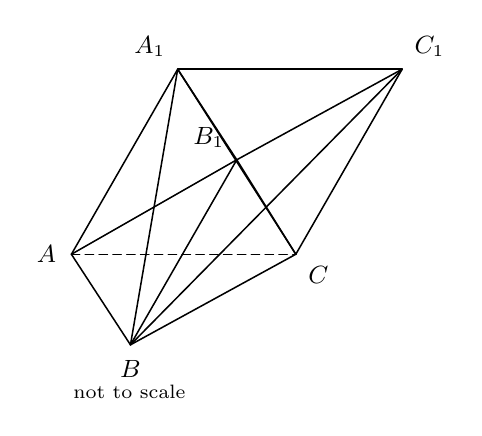
\begin{tikzpicture}[
  x=1cm,
  y=1cm,
  line cap=round,
  line join=round,
  every node/.style={font=\small},
  edge/.style={draw=black, line width=0.55pt}
]
  \coordinate (A) at (0,0);
  \coordinate (B) at (0.75,-1.15);
  \coordinate (C) at (2.85,0);
  \coordinate (A_1) at (1.35,2.35);
  \coordinate (B_1) at (2.10,1.20);
  \coordinate (C_1) at (4.20,2.35);

  % Hidden edge from the source figure.
  \draw[densely dashed, line width=0.55pt] (A) -- (C);

  % Triangular prism edges.
  \draw[edge] (A) -- (B);
  \draw[edge] (B) -- (C);
  \draw[edge] (A) -- (A_1);
  \draw[edge] (B) -- (B_1);
  \draw[edge] (C) -- (C_1);
  \draw[edge] (A_1) -- (B_1);
  \draw[edge] (B_1) -- (C_1);
  \draw[edge] (A_1) -- (C_1);

  % Additional lines appearing in the source geometry diagram.
  \draw[edge] (A_1) -- (B);
  \draw[edge] (A) -- (B_1);
  \draw[edge] (B) -- (C_1);
  \draw[edge] (A_1) -- (C);
  \draw[edge] (B_1) -- (C);

  \node[left=2pt] at (A) {$A$};
  \node[below=2pt] at (B) {$B$};
  \node[below right=1pt] at (C) {$C$};
  \node[above left=1pt] at (A_1) {$A_1$};
  \node[above left=1pt] at (B_1) {$B_1$};
  \node[above right=1pt] at (C_1) {$C_1$};
  \node[font=\scriptsize, anchor=west] at (-0.1,-1.75) {not to scale};
\end{tikzpicture}
\end{center}
\nopagebreak[4]
\Needspace{4\baselineskip}
\textbf{解析}

\Needspace{5\baselineskip}
令 $a=1$ 作尺度归一化，设底面
\nopagebreak[4]
\[
A=(0,0,0),\quad C=(1,0,0),\quad B=(1/2,\sqrt3/2,0).
\]
\Needspace{5\baselineskip}
因为侧面 $A_1ACC_1$ 垂直底面且含 $AC$，可设 $A_1=(u,0,v)$，并有 $u^2+v^2=1$。由 $A_1B=\sqrt6/2$ 得
\nopagebreak[4]
\[
(u-1/2)^2+3/4+v^2=3/2
\quad\Longrightarrow\quad u=1/2,\quad v=\sqrt3/2,
\]
\Needspace{5\baselineskip}
其中取正号仅对应图形朝向，翻转不影响所求。棱柱平移向量为 $(1/2,0,\sqrt3/2)$，故
\nopagebreak[4]
\[
B_1=(1,\sqrt3/2,\sqrt3/2),\qquad C_1=(3/2,0,\sqrt3/2).
\]
\textbf{(1) 解}

\Needspace{5\baselineskip}
$\overrightarrow{AC}=(1,0,0)$、$\overrightarrow{BC_1}=(1,-\sqrt3/2,\sqrt3/2)$，于是
\nopagebreak[4]
\[
\cos\angle(AC,BC_1)=\frac{1}{\sqrt{1+3/4+3/4}}
=\sqrt{\frac25}=\frac{\sqrt{10}}5.
\]
\textbf{(2) 解}

$\overrightarrow{A_1B}=(0,\sqrt3/2,-\sqrt3/2)$。它分别与平面 $AB_1C$ 内相交方向 $\overrightarrow{AC}=(1,0,0)$ 及 $\overrightarrow{AB_1}=(1,\sqrt3/2,\sqrt3/2)$ 点积为 $0$，故 $A_1B\perp$ 面 $AB_1C$。尺度恢复为任意 $a>0$ 后结论不变。

\gkanswer{答案（1）：$\cos\angle(AC,BC_1)=\dfrac{\sqrt{10}}5$。}

\gkanswer{答案（2）：$A_1B\perp$ 面 $AB_1C$。}

\end{answer}
\begin{answer}
\gksolhead{21}{}

\textbf{题目}：

已知盒中有 $10$ 个灯泡，其中 $8$ 个正品，$2$ 个次品。现需要从中取出 $2$ 个正品，每次取出 $1$ 个，取出后不放回，直到取出 $2$ 个正品为止。设 $\xi$ 为取出的次数，求 $\xi$ 的分布列及 $E\xi$。

\Needspace{4\baselineskip}
\textbf{解析}

\Needspace{5\baselineskip}
$\xi$ 只能取 $2,3,4$。前两次均为正品的概率为
\nopagebreak[4]
\[
P(\xi=2)=\frac8{10}\frac7{9}=\frac{28}{45}.
\]
\Needspace{5\baselineskip}
若恰在第三次取到第二个正品，则前三次恰有一件次品，且第三次为正品：
\nopagebreak[4]
\[
P(\xi=3)=\left(\frac8{10}\frac2{9}+\frac2{10}\frac8{9}\right)\frac7{8}
=\frac{14}{45}.
\]
\Needspace{5\baselineskip}
$\xi=4$ 时前三次恰有一件正品、两件次品，其概率为
\nopagebreak[4]
\[
P(\xi=4)=3\cdot\frac8{10}\frac2{9}\frac1{8}=\frac{1}{15}.
\]
\Needspace{5\baselineskip}
三概率之和 $28/45+14/45+1/15=1$。因此
\nopagebreak[4]
\[
E\xi=2\frac{28}{45}+3\frac{14}{45}+4\frac{1}{15}=\frac{22}{9}.
\]

\gkanswer{答案：$P(\xi=2)=\dfrac{28}{45}$，$P(\xi=3)=\dfrac{14}{45}$，$P(\xi=4)=\frac{1}{15}$；$E\xi=\dfrac{22}{9}$}

\end{answer}
\begin{answer}
\gksolhead{22}{}

\textbf{题目}：

已知抛物线 $C:y=x^2+4x+\dfrac{2}{7}$，过 $C$ 上一点 $M$，且与 $M$ 处的切线垂直的直线称为 $C$ 在点 $M$ 的法线。

(1) 若 $C$ 在点 $M$ 的法线的斜率为 $-\dfrac{1}{2}$，求点 $M$ 的坐标 $(x_0,y_0)$；

(2) 设 $P(-2,a)$ 为 $C$ 对称轴上的一点，在 $C$ 上是否存在点，使得 $C$ 在该点的法线通过点 $P$？若有，求出这些点，以及 $C$ 在这些点的法线方程；若没有，请说明理由。

\Needspace{4\baselineskip}
\textbf{解析}

令 $s=x_0+2$，则曲线可写为 $y=s^2-26/7$，切线斜率为 $2s$。当 $s\ne0$ 时法线斜率为 $-1/(2s)$；顶点 $s=0$ 处切线水平，法线为竖直线 $x=-2$。

\textbf{(1) 解}

$-1/(2s)=-1/2$ 给出 $s=1$，即 $x_0=-1$，$y_0=1-4+2/7=-19/7$。

\textbf{(2) 解}

\Needspace{5\baselineskip}
顶点法线 $x=-2$ 对任意 $P(-2,a)$ 都成立，顶点 $M=(-2,-26/7)$。其余法线取 $s\ne0$，令其通过 $P$：
\nopagebreak[4]
\[
a=s^2-\frac{26}{7}+\frac12=s^2-\frac{45}{14},
\qquad s^2=a+\frac{45}{14}.
\]
\Needspace{5\baselineskip}
故仅当 $a>-\frac{45}{14}$ 时有两个非顶点点，$s=\pm\sqrt{a+45/14}$，对应
\nopagebreak[4]
\[
M=\left(-2\pm\sqrt{a+\frac{45}{14}},\ a-\frac12\right),\qquad
y-a=\mp\frac{x+2}{2\sqrt{a+\frac{45}{14}}}.
\]
当 $a=-45/14$ 时只得到顶点，该法线已计入；当 $a<-45/14$ 时方程无实根。特别地，顶点处不能套用有限斜率公式，否则会漏掉对所有 $a$ 均存在的竖直法线。

\gkanswer{答案（1）：$M=(-1,-\dfrac{19}{7})$。}

\gkanswer{答案（2）：对任意 $a$，顶点 $M=(-2,-\dfrac{26}{7})$ 处的竖直法线 $x=-2$ 均通过 $P$。若 $a>-\dfrac{45}{14}$，另有两点 $M=(-2\pm\sqrt{a+\dfrac{45}{14}},a-\dfrac12)$，法线为 $y-a=\mp\dfrac{x+2}{2\sqrt{a+\dfrac{45}{14}}}$；若 $a\le-\dfrac{45}{14}$，没有其他点。}

\end{answer}